\section{Projection mapping}\label{sec:projection-mapping}

Projection mapping is a spatial augmented reality \cite{Bimber2005} technique in which video projectors are used to overlay virtual geometry on top of real objects or surfaces. This allows to create an immersive environment that together with 3D perception systems can be used to develop interactive interfaces that show contextual information for helping or teaching human operators performing complex tasks faster. The next sections describe the mathematical projector modeling and the associated calibration that is necessary for performing proper 3D rendering of the virtual world in order to achieve high accuracy projection.


\subsection{Projector modeling}

Over the years, several projection technologies were developed according to the requirements of color fidelity / saturation, image sharpness, brightness, contrast, refresh rate and price. Currently, the video projection market is split between reflective \gls{dlp} and transmissive \gls{lcd} projection technology, with a small percentage of projectors consisting of a hybrid between the two technologies (\gls{lcos}).

For video projection mapping purposes \cite{Raskar1998,Bimber2005,Tan2013,Fujimoto2014}, reflective projectors are better suited than the remaining technologies given their ability to create images with smaller gaps between the projected pixels (smoother images) and they also have higher contrast, better color accuracy / uniformity, much fewer dead pixels and the image quality does not degrade over time. The main stages of the image creation in a \gls{dlp} projector are show in \cref{fig:dlp-projector-diagram-dmd}. The first phase is the generation of light from either a lamp or a \gls{led} / laser array, which is later on condensed on a lens in order to pass through a moving color wheel to become one of the 3 primary additive colors (red, green, blue). The colored light then passes through a shaping lens and hits a \gls{dmd} which has an electronic controllable mirror for each projection pixel that either reflects the light into the projection lens or into a heat sink. Color shading is achieved by controlling how long and how often the micro mirrors in the \gls{dmd} are reflecting each light color into the lens (or into the heat sink).

The mathematical modeling of a \gls{dlp} projector can be seen as an inverse pinhole camera \cite{Hartley2003} (shown in \cref{fig:camera-intrinsics}), given the grid disposition of the mirrors in the \gls{dmd} and the very low distortion that modern \gls{dlp} projectors have. As such, scene rendering can be performed efficiently using the \gls{opengl} projection matrix (shown in \cref{eq:projection-matrix,eq:ndc-matrix,eq:perspective-matrix}), which incorporates the focal lengths (Fx, Fy), principal point (Cx, Cy) and axis skew (S) intrinsic camera parameters (in pixel units). The correction of lens distortion for \gls{dlp} projectors typically uses 3 coefficients for removing radial distortions and 2 coefficients for accounting for the tangential distortions.


\begin{figure}[H]
	\begin{floatrow}[2]
		\ffigbox[\FBwidth]
		{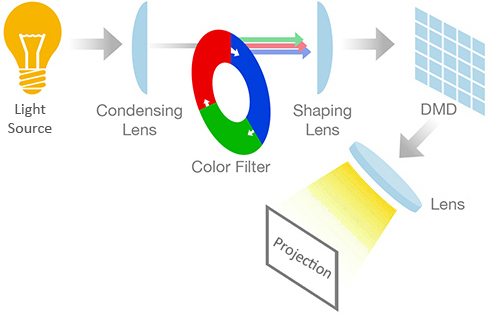
\includegraphics[height=.19\textheight]{dlp-projector-diagram-dmd}}
		{\caption[Single chip \glsentrytext{dlp} diagram]{Single chip \glsentrytext{dlp} diagram\protect\footnotemark}\label{fig:dlp-projector-diagram-dmd}}
		\ffigbox[\FBwidth]
		{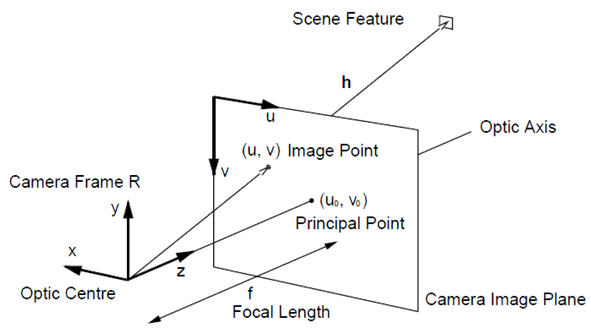
\includegraphics[height=.19\textheight]{camera-intrinsics}}
		{\caption[Pinhole camera model]{Pinhole camera model\protect\footnotemark}\label{fig:camera-intrinsics}}
	\end{floatrow}
\end{figure}
\footnotetext[\the\numexpr\value{footnote}-1\relax]{\url{https://vimeo.com/blog/post/display-tech-home-projectors}}
\footnotetext[\value{footnote}]{\url{http://perso.ensta-paristech.fr/~filliat/Courses/2011_projets_C10-2/BRUNEAU_DUBRAY_MURGUET/monoSLAM_bruneau_dubray_murguet_en.html}}


{
	\scriptsize
	\begin{equation}\label{eq:projection-matrix}
	ProjectionMatrix = \glsentrytext{ndc}Matrix \times PerspectiveMatrix
	\end{equation}
	
	\begin{equation}\label{eq:ndc-matrix}
	NDCMatrix = 
	\begin{bmatrix}
	\frac{2}{ImageWidth} & 0 & 0 & -1 \\
	0 & \frac{2}{ImageHeight} & 0 & -1 \\
	0 & 0 & \frac{-2}{ClipFar - ClipNear} & \frac{-(ClipFar + ClipNear)}{ClipFar - ClipNear} \\
	0 & 0 & 0 & 1
	\end{bmatrix}
	\end{equation}
	
	
	\begin{equation}\label{eq:perspective-matrix}
	PerspectiveMatrix = 
	\begin{bmatrix}
	Fx & S & -Cx & 0 \\
	0 & Fy & -Cy & 0 \\
	0 & 0 & ClipNear + ClipFar & ClipNear \times ClipFar \\
	0 & 0 & -1 & 0
	\end{bmatrix}
	\end{equation}
}


\subsection{Projector calibration}

High accuracy projection mapping requires proper hardware / software calibration of the camera / projector and also appropriate positioning within the intended workspace in order to avoid occlusions caused by the objects 3D shape or the human operators. This calibration aims to compute the intrinsic parameters of the projector (that do not change when the projector is moved within the workspace) along with the extrinsic parameters that are needed to know where is the projector in the global reference frame in order to be able to do proper 3D rendering of the scene that will be projected.

The intrinsic parameters of a \gls{dlp} projector can be computed using image analysis of complementary gray code patterns (example in \cref{fig:dlp-calibration-pattern-wall}) projected into a chessboard. The calibration system proposed in \cite{Moreno2012} was used to retrieve the 5 intrinsic parameters (Fx, Fy, Cx, Cy, S) of the projector along with the 3D position and rotation of the projector in relation to the camera (that remains firmly attached to the projector support for fast recalibration of the extrinsic parameters). It was used 5 sets of 42 gray code image patterns captured with the chessboard in different positions and orientations in relation to the projector, that was pointing to the table workspace at a distance of 0.81 meters. After calibration, it was projected a validation pattern to evaluate the accuracy of the projection, and as can be seen in \cref{fig:dlp-projected-chessboard}, the white squares were projected into the chessboard with sub-millimeter accuracy.

\begin{figure}[H]
	\begin{floatrow}[2]
		\ffigbox[\FBwidth]
		{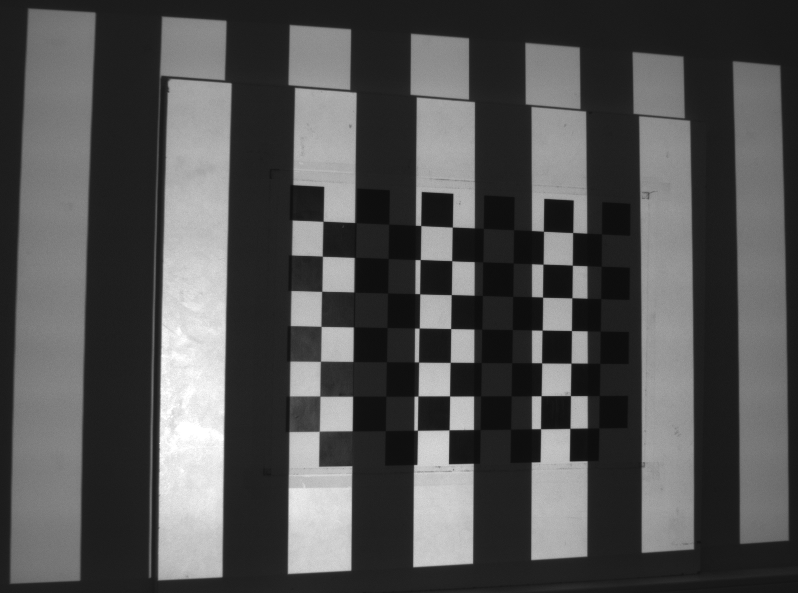
\includegraphics[height=.205\textheight]{dlp-calibration-pattern-wall}}
		{\caption{One of the \glsentrytext{dlp} projector calibration patterns}\label{fig:dlp-calibration-pattern-wall}}
		\ffigbox[\FBwidth]
		{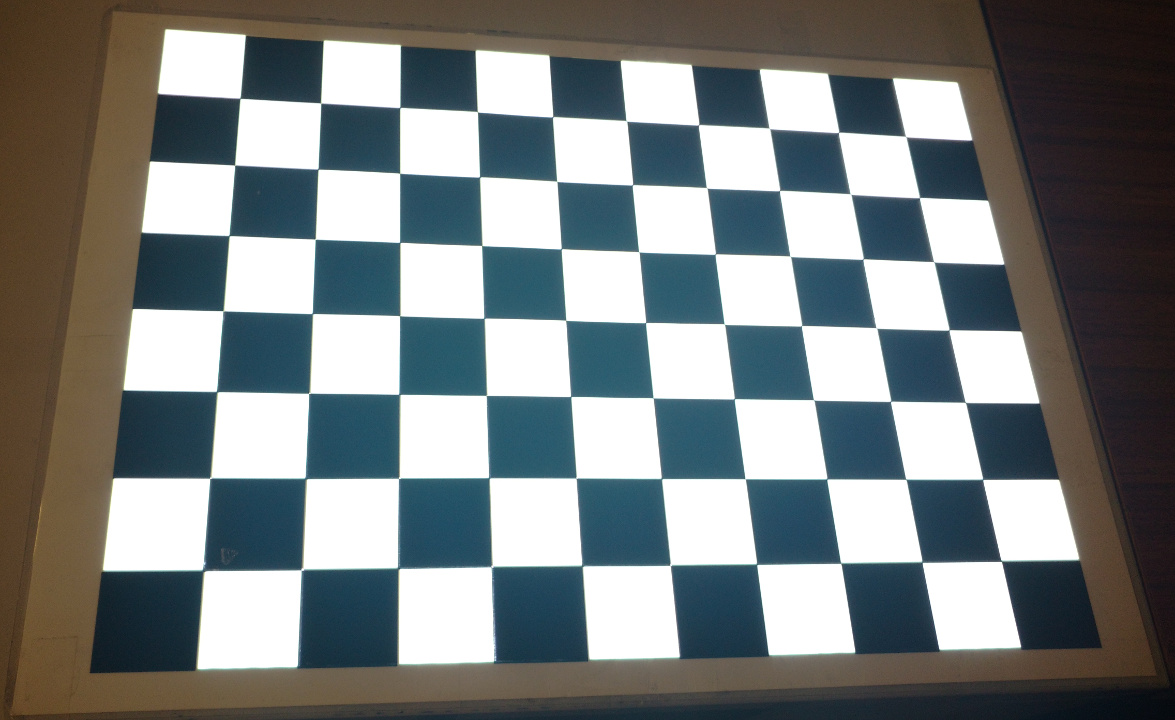
\includegraphics[height=.205\textheight]{chessboard}}
		{\caption{\glsentrytext{dlp} projector validation pattern}\label{fig:dlp-projected-chessboard}}
	\end{floatrow}
\end{figure}

After having the intrinsic parameters of the camera and projector along with the relative position of the projector in relation to the camera, computing the global position of the projector in relation to the chessboard reference frame can be done by multiplying the $4 \times 4$ homogeneous matrix that gives the transformation from the chessboard origin (shown in \cref{fig:chess-board-detection}) to the camera frame, with the $4 \times 4$ homogeneous matrix that gives the transformation from the camera frame to the projector frame.

\begin{figure}[H]
	\centering
	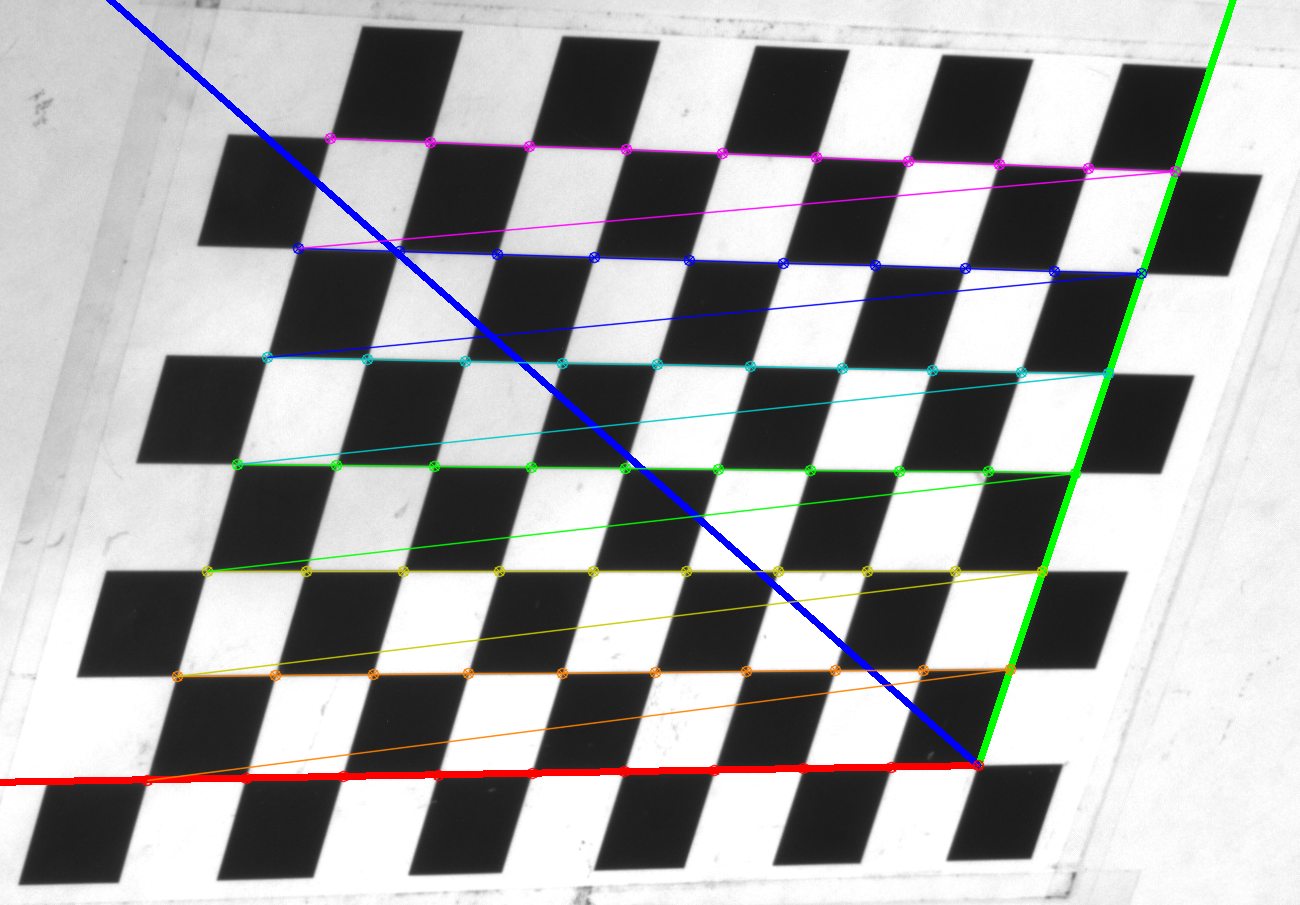
\includegraphics[width=0.47\linewidth]{chess-board-detection}
	\caption{Camera pose estimation in relation to the chessboard origin (using the Kinect 2 RGB camera)}
	\label{fig:chess-board-detection}
\end{figure}


\subsection{Scene rendering}

For achieving accurate projection mapping, the Gazebo simulator\footnote{\url{http://gazebosim.org}} camera implementation was improved to allow the setting of a custom projection matrix in order to perform 3D rendering with a camera model that takes into account the projector intrinsic parameters. Moreover, it was added the possibility to dynamically change image, video and text during runtime for allowing the display of the relevant information for each assembly step.
For efficient 3D scene rendering, the Gazebo simulator relies on the cross platform open source Ogre3D graphics engine\footnote{\url{http://www.ogre3d.org}}, that in turn uses the \gls{opengl} \gls{gpu} \gls{api} to take advantage of the massively parallel graphics cards currently available to generate raster images for the \gls{dlp} projector (example of a rendered scene for the last assembly step in \cref{fig:scene-rendering}).

For user interface, the Gazebo simulator has a Qt\footnote{\url{https://www.qt.io/}} \gls{gui} that allows visual inspection of the scene while also giving the option to add new objects or move and rotate existing models. Moreover, for lightweight rendering, it can also start in server mode without a \gls{gui}.

\begin{figure}
	\centering
	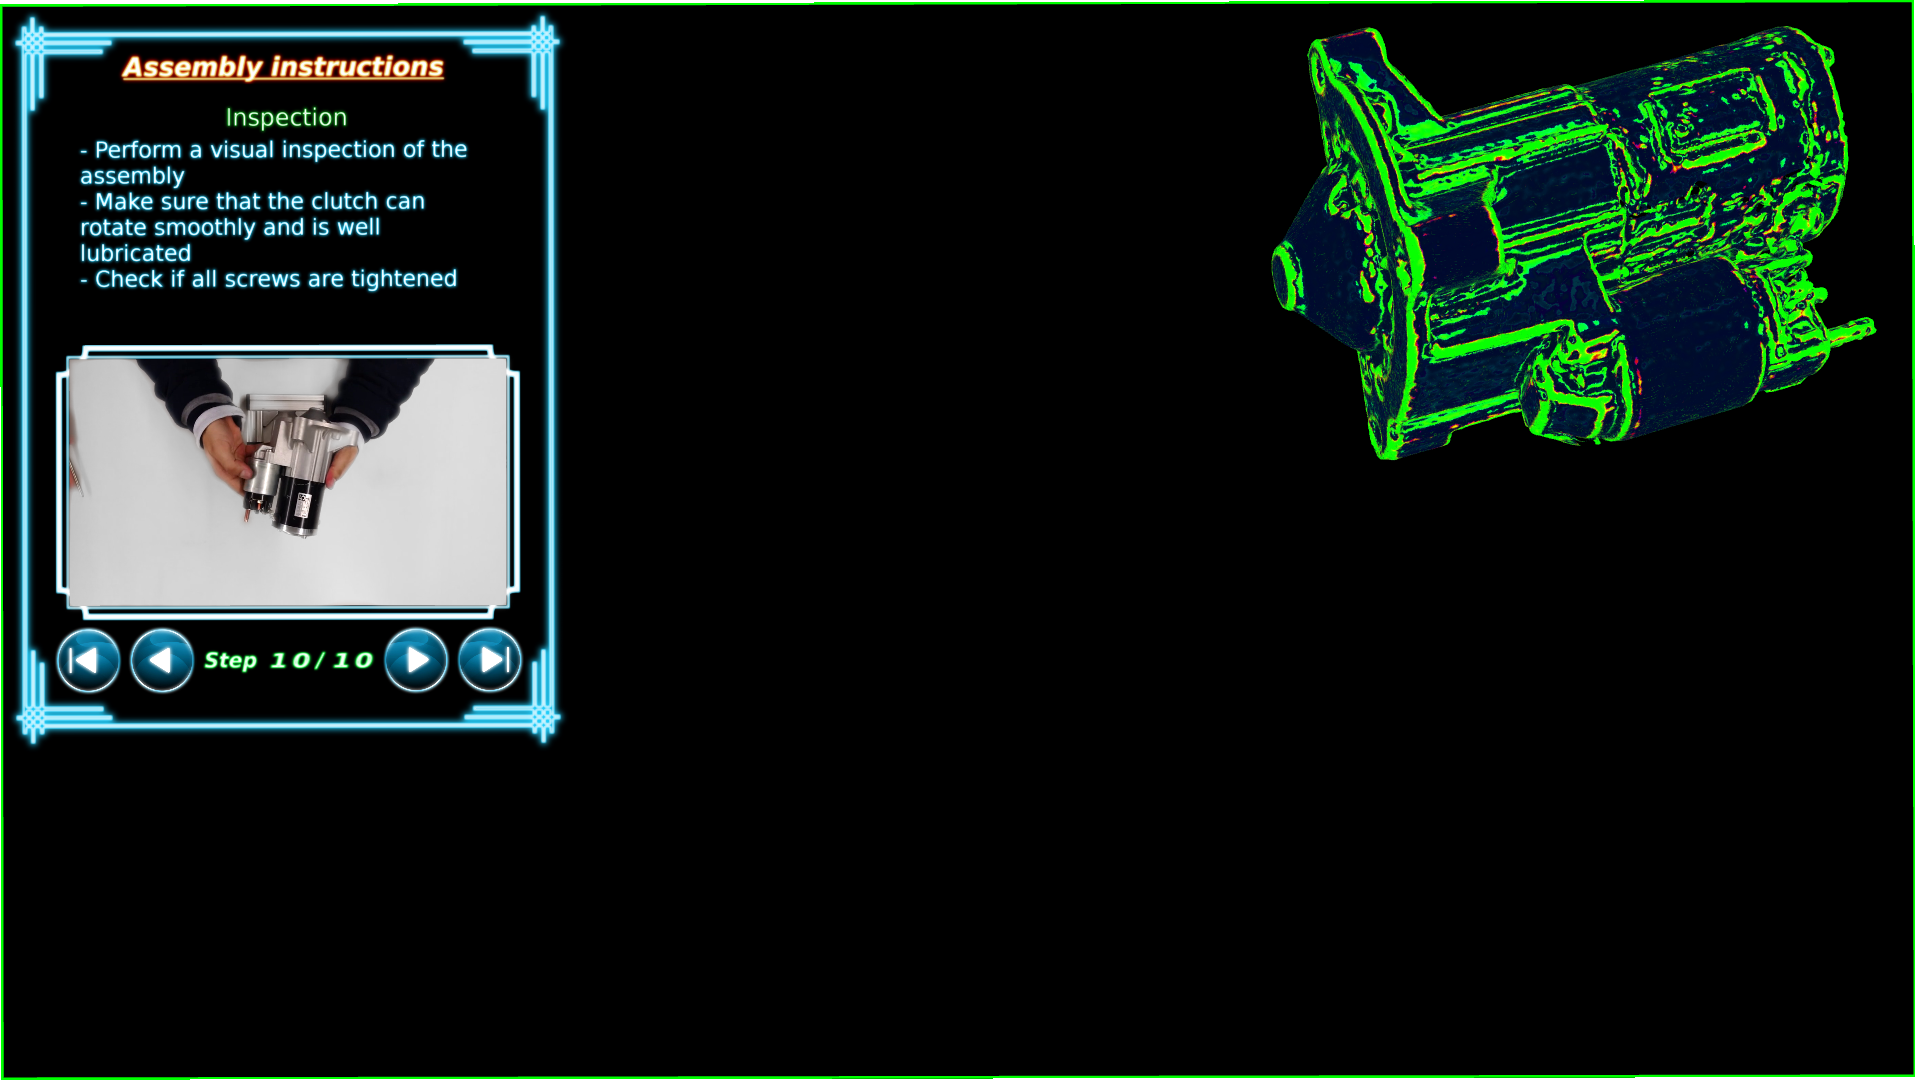
\includegraphics[width=0.8\linewidth]{scene-rendering}
	\caption{3D scene rendering using the Gazebo simulator}
	\label{fig:scene-rendering}
\end{figure}



\section{Human machine interaction}\label{sec:human-machine-interaction}

The immersive \gls{hmi} system developed (shown in \cref{fig:scene-rendering,fig:human-machine-interface}) projects into the workspace detailed textual information of the current assembly task along with a video showing the operation being performed by an expert operator. Given the high variability of assembly / maintenance operations, the system was designed to decompose the assembly process into a set of small and concise operations. This allows to keep the operator focused on the current task and reduces the required projection area. Moreover, the operator can pause and move the video forwards and backwards, allowing to inspect a given complex operation with more time.

The user interaction with the projected \gls{hmi} is done by analyzing the 3D point cloud sensor data that falls within a set of \glspl{roi} (shown in \cref{fig:interaction-rois}). When a minimum number of points falls within a given \gls{roi}, the cluster of points centroid is extracted (shown as spheres in \cref{fig:interaction-rois}) and if this \gls{roi} is associated with a button, the user needs to hold the finger for at least 0.25 seconds to trigger the action. Moreover, to avoid unintentional action triggering, the user needs to remove and insert the finger into the \gls{roi} to request the action again. On the other hand, if the \gls{roi} is associated with the video seek bar \gls{roi} (the vertical yellow box in \cref{fig:interaction-rois}), the video seek time is computed considering the relative position of the finger within the \gls{roi} (the bottom of the \gls{roi} is associated with the start of the current video while the top corresponds to the end of the current video).

Besides video play / pause functionality (provided by the blue middle \gls{roi} shown in \cref{fig:interaction-rois}), the \gls{hmi} also allows the operator to navigate within the assembly operations (using the green \glspl{roi} visible in \cref{fig:interaction-rois}). As can be seen in \cref{fig:human-machine-interface,fig:interaction-rois}, there are buttons for moving to the first, previous, next and last assembly step. Moreover, it is also shown what is the number of the current assembly step and how many steps are required to complete the assembly.

\begin{figure}[H]
	\begin{floatrow}[2]
		\ffigbox[\FBwidth]
		{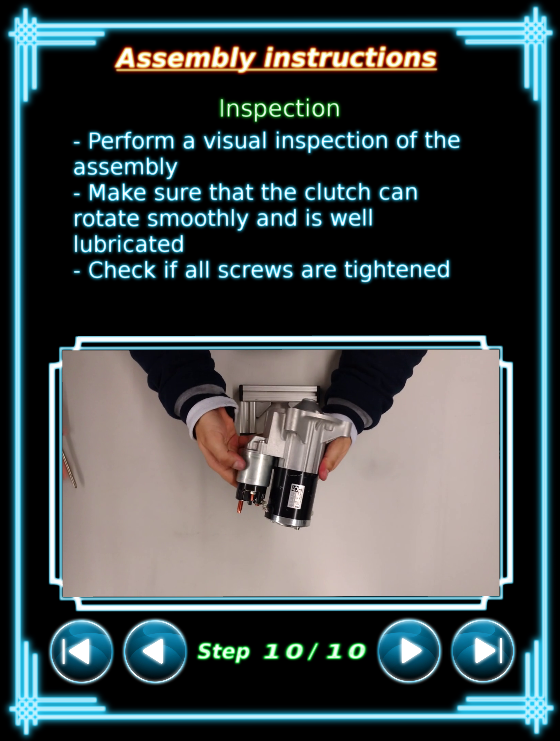
\includegraphics[height=.35\textheight]{human-machine-interface}}
		{\caption{Rendering of the human machine interface}\label{fig:human-machine-interface}}
		\ffigbox[\FBwidth]
		{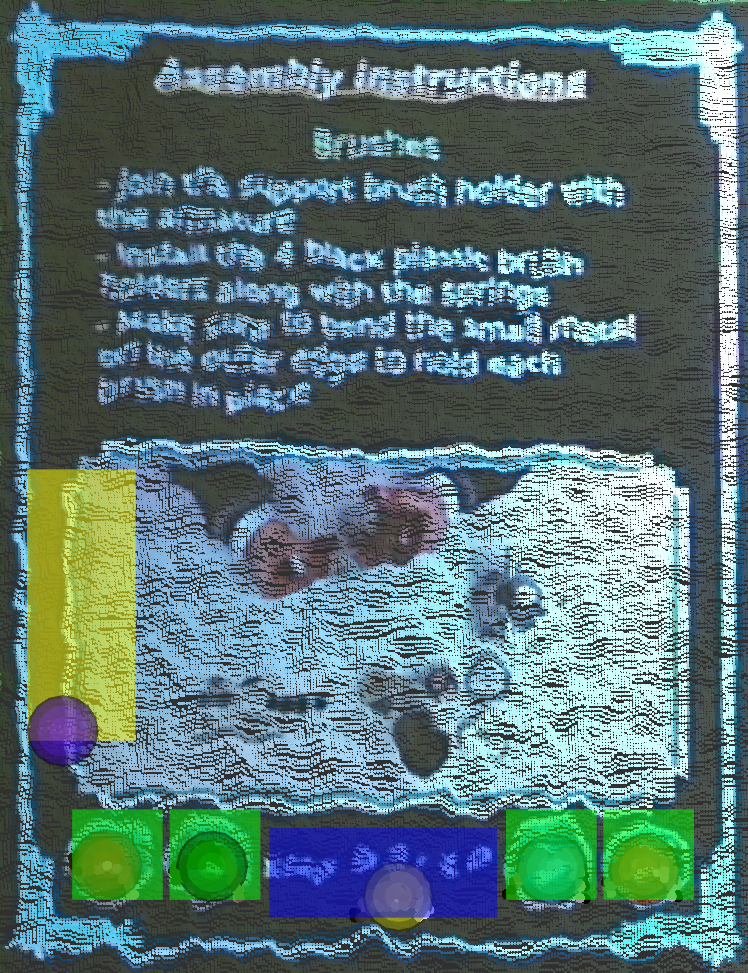
\includegraphics[height=.35\textheight]{interaction-rois}}
		{\caption{\glspl{roi} for the \gls{hmi} (overlaid on top of the Kinect 2 point cloud sensor data)}\label{fig:interaction-rois}}
	\end{floatrow}
\end{figure}


\section{Object 3D reconstruction}\label{sec:object-reconstruction}

The last step of the assembly process is a visual inspection by the operator of the final product in order to ensure that every part was mounted correctly. To speedup this analysis the projection mapping system projects into the workspace the expected product outline (generated by colorizing the mesh using the surface curvature information). To be able to perform proper 3D rendering and also to detect and track the object within the workspace, it is necessary the 3D \gls{cad} model of the final product. Given the lack of public available \gls{cad} models for the Mitsubishi M000T20873 starter motor (shown in \cref{fig:starter-motor}), it was necessary to perform object 3D reconstruction. The 3D mesh model shown in \cref{fig:object-reconstruction} was generated using the David Laser 3D structured light system\footnote{\url{http://www.david-3d.com}}, and was built by surface matching algorithms using sensor data retrieved from 38 scans in which the starter motor was moved and rotated several times in order to capture enough sensor data to be able to reconstruct the entire surface. This particular object created some challenges for the structured light scanner, given that it has polished metallic sections and also black coated regions. As such, it was necessary to capture the same object sections several times with different projector brightness and camera exposure times (the dark regions required the maximum projector brightness and very high exposure times while the polished sections required dimmer projector brightness and very short exposure times in order for the surface to be fully reconstructed).

\begin{figure}[H]
	\begin{floatrow}[2]
		\ffigbox[\FBwidth]
		{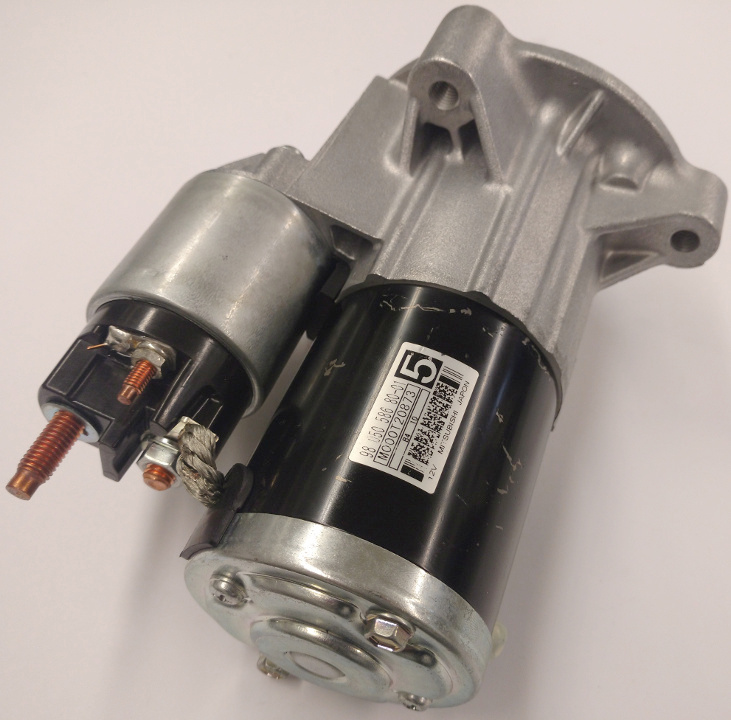
\includegraphics[height=.136\textheight]{mitsubishi-m000t20873-front}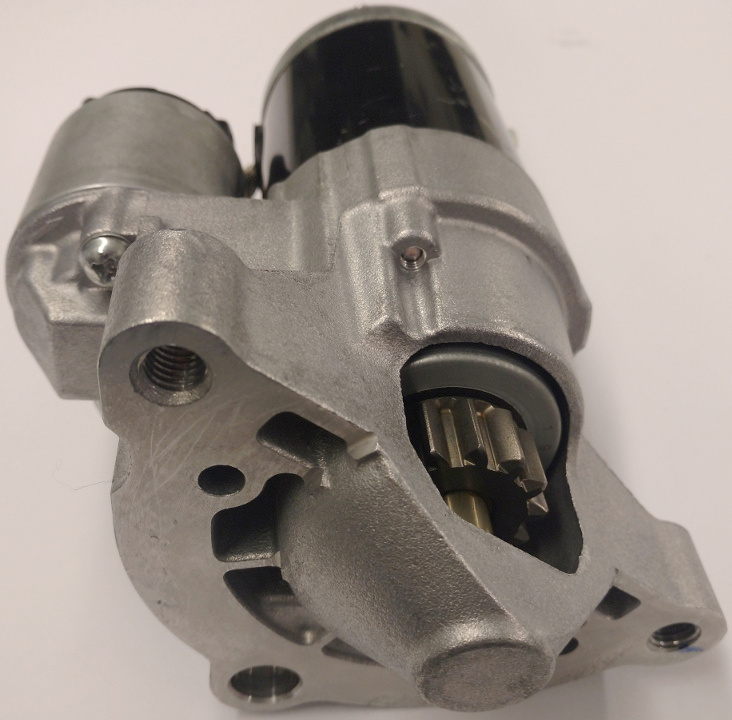
\includegraphics[height=.136\textheight]{mitsubishi-m000t20873-back}}
		{\caption{Mitsubishi M000T20873 starter motor}\label{fig:starter-motor}}
		\ffigbox[\FBwidth]
		{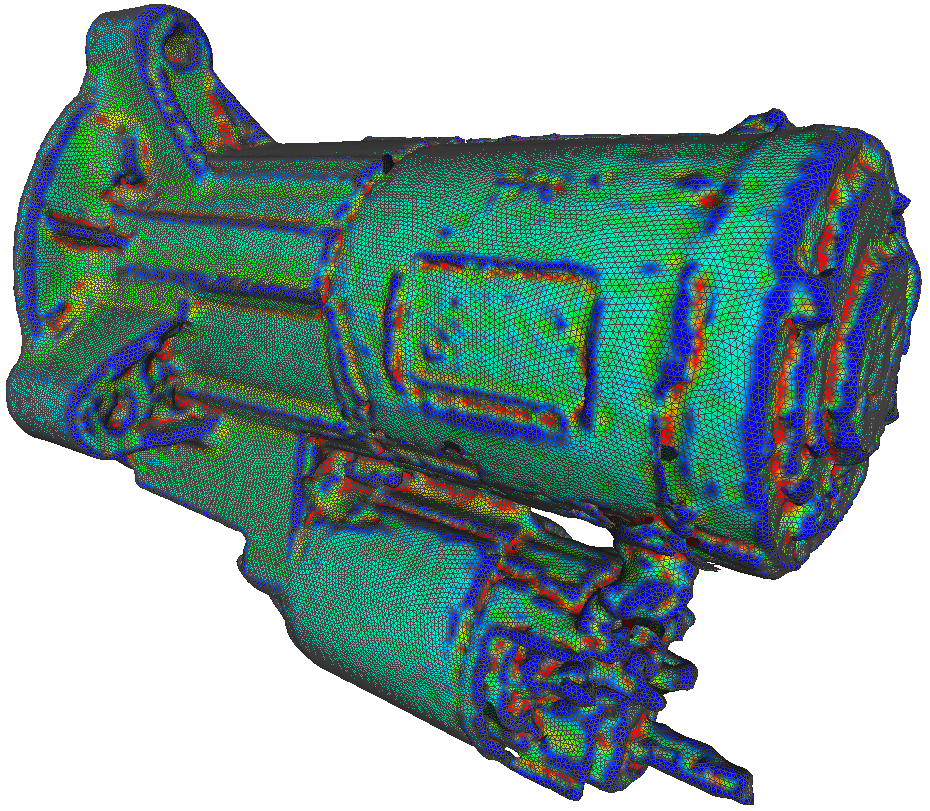
\includegraphics[height=.136\textheight]{object-reconstruction-front}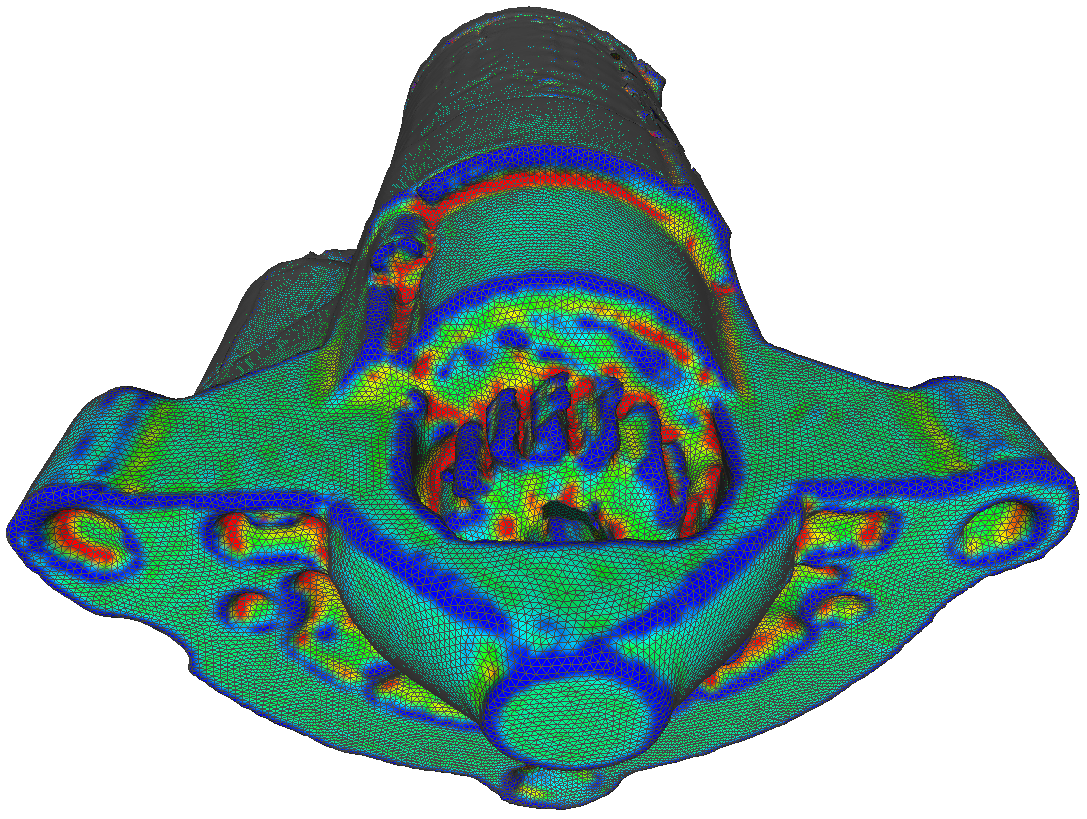
\includegraphics[height=.136\textheight]{object-reconstruction-back}}
		{\caption{3D model of the starter motor reconstructed using a structured light scanner}\label{fig:object-reconstruction}}
	\end{floatrow}
\end{figure}



\section{Object recognition}\label{sec:object-recognition}

Robust and accurate object recognition and pose estimation is a requirement when developing projection mapping systems with dynamic objects. This is one of the most challenging perception tasks, which has received a lot of research over the years, both at the hardware and software level. The next sections describe the main processing stages of the robot localization system (described in \cite{Costa2016}) that was reconfigured and improved to perform 3D object recognition.


\subsection{Reference models}

The first step in any perception system is the definition of the geometry of the object that we intend to recognize. As such, given a \gls{cad} / mesh model, the object recognition system generates the respective point cloud and the associated keypoints and feature descriptors.


\subsection{Point cloud assembly}

The object recognition system can use any sensor that provides point clouds, namely RGB-D / \gls{tof} cameras, \glspl{lidar}, stereo vision systems among many others. Each of these types of sensors have very different operation rates and measurement accuracy. As such, the recognition system allows the assembly of several sensor scans using a circular buffer in order to reduce the impact of sensor noise and increase the observed surface area of the objects.


\subsection{Filtering and down sampling}

The time it takes to perform cloud registration increases considerable as the amount of points in the sensor point cloud and in the reference model becomes larger. As such, adjusting the level of detail of the point clouds by using voxel grids and random sampling gives some control over the desired pose estimation accuracy and the computational resources that will be required. Moreover, when we know the expected workspace, we can crop the sensor data to a given \gls{roi} (such as a given volume above the working table), which removes any unnecessary environment clutter, resulting in a preliminary segmentation of the sensor data that later will be analyzed for object recognition. This stage is also useful to mitigate the measurement errors of the depth sensors, since the centroid of a voxel that contains points from several scans will be closer to the real surface (if the voxels have dimensions slightly larger than the expected measurement errors).


\subsection{Normal estimation}

Most of feature detection, description and matching algorithms along with some registration methods rely on the point's surface normal and curvature. These algorithms analyze the neighborhood of a given point in order to compute the surface normal, and as such, the correct specification of what points should be included in the estimation is crucial to achieve accurate results. This depends on the environment geometry and the level of detail that is required, and is usually done by specifying a radius distance or by limiting the number of neighboring points to use.


\subsection{Keypoint detection}

Aligning two point clouds with overlapping views of the environment requires the establishment of point correspondences. If both point clouds have similar sensor origins, these can be determined with nearest neighbor's searches and filtered with correspondence rejectors (using other point properties such as reflectance and color). But if they were acquired in two very different positions, then more advanced techniques must be employed.

One of those techniques uses histograms to describe the geometric properties of the environment around a given point. This allows points to be matched even if they have completely different Euclidean coordinates. Also, by using histograms and sampling techniques, these descriptors are much more robust against sensor noise and varying level of point density. However, these advantages come with a heavy computational cost, and as such, point descriptors should only be computed on the most descriptive areas of the environment.

Identifying these environment points is known as feature / keypoint detection \cite{Filipe2014}, and usually involves finding interesting points, such as corners and edges. Besides uniqueness, these points must also be repeatable. This means that the detection algorithms should be able to find the same points even if they are present in different point clouds with sensor noise and varying point density. This is of the utmost importance, because if the same keypoints are not identified on both clouds, then matching the point descriptors will likely fail.

The object recognition systems used the \gls{sift} \cite{Lowe2004} algorithm on the point's curvature, but it also supports the \gls{iss3d} \cite{Zhong2009} keypoint detector on the point's normals.


\subsection{Keypoint description}

Describing a keypoint usually involves analyzing its neighboring points and computing a given metric or histogram that quantifies the neighbor's relative spatial distribution, their normals angular relation, associated geometry or other metrics that are deemed useful. Several approaches were suggested over the years according to different recognition needs and they are the basis of feature matching algorithms used in the initial pose estimation.

The object recognition system used the \gls{fpfh} \cite{Rusu2009} keypoint descriptor, but it also supports the \gls{pfh} \cite{Rusu2008a}, the \gls{shot} \cite{Tombari2011}, the \gls{sc3d} \cite{Frome2004}, the \gls{usc} \cite{Tombari2010} and the \gls{esf} \cite{Wohlkinger2011}.


\subsection{Cloud registration}

Point cloud registration is the process of finding the transformation matrix (usually translation and rotation only) that when applied to a given ambient cloud will minimize an error metric (such as the mean square error of the ambient point cloud in relation to a given reference point cloud). Several approaches were suggested over the years and they can be categorized as point or feature cloud registration.


\subsubsection{Initial alignment with keypoints descriptor matching}\label{subsec:localization-system_feature-registration}

Feature registration is the process of matching keypoint descriptors in order to find an initial alignment between two point clouds. The object recognition system uses a feature registration method similar to the \gls{sacia} algorithm presented in \cite{Rusu2009}. It uses a \gls{ransac} approach to select the best registration transformation after a given number of iterations. In each iteration a subsample of randomly selected descriptors from the ambient cloud is retrieved. Then for each of these descriptors, $k$ best matching descriptors in the reference point cloud are searched (using a kd-tree) and one of them is chosen randomly. Later after having filtered these correspondences between ambient and reference descriptors, the registration matrix is computed. If this registration matrix results in a point cloud overlap that has a minimum of inliers percentage (a point in the ambient cloud is an inlier if it has a point in the reference cloud closer than a given distance), then it is considered an acceptable initial pose. In the end of all iterations, the best initial pose (if found) is refined with a point cloud registration algorithm.


\subsubsection{Final alignment with point cloud error minimization}

Point cloud registration algorithms such as \gls{icp} \cite{Besl1992} (with its several known variations \cite{Rusinkiewicz2001,Pomerleau2013} like \gls{icp} point-to-point, \gls{icp} point-to-point non-linear, \gls{icp} point-to-plane and generalized \gls{icp} \cite{Segal2009}) and the \gls{ndt} \cite{Magnusson2009} are among the most popular algorithms to register point clouds. They can achieve very accurate cloud registration but they require an approximate initial pose for the registration to successfully converge to a correct solution (otherwise they may achieve only partial cloud overlap or even fail to converge to a valid solution).

In \cref{fig:initial-pose-estimation} is shown the estimation of the pose of the starter motor. When the system started (left image), it subsampled the reference pointcloud (small green circles) and computed the keypoints (large yellow circles) and associated feature descriptors. Then, when sensor data arrived, it found the keypoints (blue circles) and their descriptors. Finally it applied the feature matching and registration refinement and achieved the pose estimation showed on the right image of \cref{fig:initial-pose-estimation} (observe the overlap between the sensor data and the reference point cloud). After the successful initial pose estimation phase, the recognition system enters in tracking mode and relies only on point cloud matching algorithms (given their better accuracy and lower computational cost). If the tracking is lost, the feature matching algorithms are used again to find a plausible estimation of the object position that is then refined with the point cloud registration refinement algorithms.

%\begin{figure}[!ht]
%	\centering
%	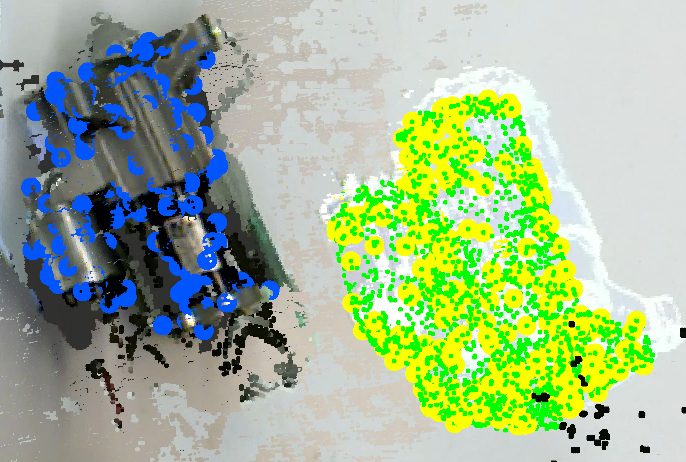
\includegraphics[height=.27\textheight]{initial-pose-estimation-1-before}
%	\hspace{0.5em}
%	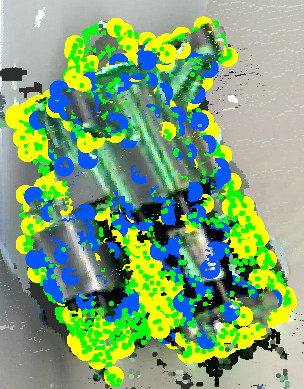
\includegraphics[height=.27\textheight]{initial-pose-estimation-1-after}
%	\caption{Initial pose estimation of assembled object}
%\end{figure}

\begin{figure}[!ht]
	\centering
	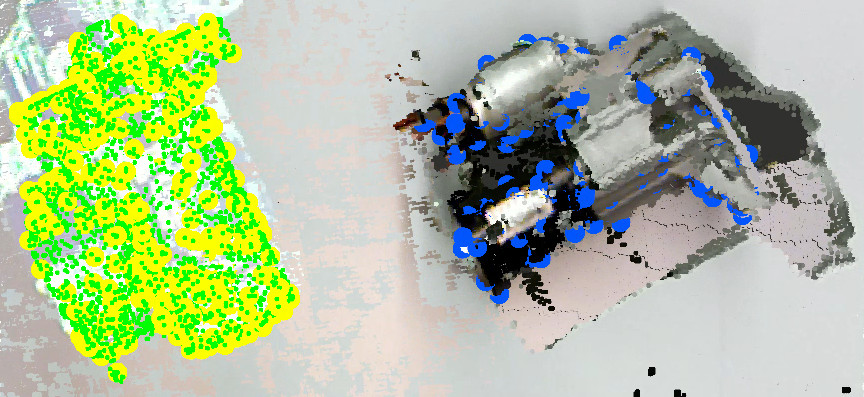
\includegraphics[height=.182\textheight]{initial-pose-estimation-2-before}
	\hspace{0.5em}
	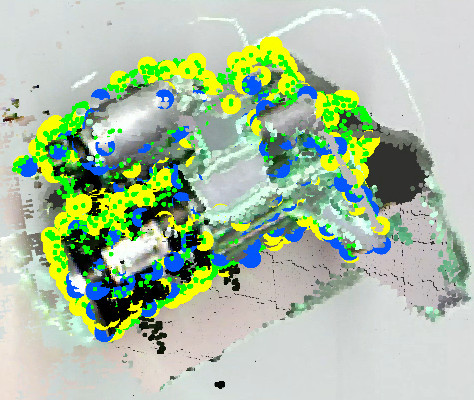
\includegraphics[height=.182\textheight]{initial-pose-estimation-2-after}
	\caption{Initial pose estimation of assembled starter motor}
	\label{fig:initial-pose-estimation}
\end{figure}


\subsection{Outlier detection}

Detecting which points from the sensor data are not part of the reference point cloud can be very useful to evaluate the quality of point cloud registration as well as to analyze if the object recognition was successful (if a high number of points were considered outliers then the object recognition is likely to have failed). It's computation splits the ambient cloud into two point sets. One containing inliers (points correctly registered and present in the reference point cloud) and the other having the outliers (points that are either incorrectly registered or not present in the reference cloud). A given ambient point can be classified as outlier if the corresponding closest point in the reference cloud is farther way than a given distance threshold. These operations can be done efficiently by using the reference point cloud kd-tree.
